\documentclass[11pt]{article}

% Change "review" to "final" for final version.
\usepackage[preprint]{acl}

% Standard packages
\usepackage{times}
\usepackage{latexsym}
\usepackage[T1]{fontenc}

\usepackage{microtype}
\usepackage{inconsolata}

% Additional packages
\usepackage{graphicx}
\usepackage{booktabs}
\usepackage{multirow}
\usepackage{amsmath}
\usepackage{url}
\usepackage{tikz}
\usetikzlibrary{arrows.meta, positioning, shapes.geometric}

\title{A Multi-task Learning Approach for Vietnamese Complaint Detection and Complaint Span Extraction in E-commerce Reviews}

\author{
\begin{tabular}{c}
\textbf{Vu Ngoc Bao Thang} \quad
\textbf{Do Luong Phuong Sang} \quad
\textbf{Le Viet Tan} \quad
\textbf{Luu Minh Tan} \\
University of Information Technology, VNU-HCM \\
Vietnam National University, Ho Chi Minh City \\
\end{tabular}
}

\begin{document}
\maketitle

\begin{abstract}
Online reviews on e-commerce platforms contain valuable information about customer satisfaction and product-related issues. In Vietnamese e-commerce, complaint detection is challenging due to informal language, spelling variations, mixed sentiments, and implicit expressions of dissatisfaction. Previous studies mainly focus on classifying whether a review contains a complaint, but they do not identify which part of the review expresses the complaint.

In this work, we propose a PhoBERT-based multi-task learning approach for Vietnamese complaint analysis. The model jointly performs two tasks: complaint classification and complaint span extraction. PhoBERT-base-v2 is used as the shared encoder, followed by a classification head for binary complaint detection and a sequence labeling head with CRF for BIO-based complaint span extraction. We evaluate the proposed approach on a Shopee review dataset and a manually annotated BIO subset for complaint extraction.

Experimental results show that TF-IDF-based LinearSVM achieves strong performance for complaint classification, with a Macro-F1 score of 0.9428 and Complaint-F1 of 0.9470. For the NER task, single-task PhoBERT-based models perform poorly due to limited BIO-annotated data, achieving Entity-F1 scores of around 0.02. In contrast, the proposed multi-task PhoBERT + CRF model improves Entity-F1 to 0.3279 and Token-F1 to 0.6627 under different alpha configurations. These results suggest that multi-task learning can help improve complaint span extraction when labeled NER data is limited.
\end{abstract}

\section{Introduction}

Online customer reviews have become an important source of user-generated content on e-commerce platforms. These reviews reflect customer satisfaction, product quality, delivery experience, packaging issues, and after-sales service. Among them, complaint reviews are particularly valuable because they directly indicate problems that sellers and platforms need to address. Automatically detecting complaints from large-scale review data can support customer service, product quality monitoring, and business decision-making.

Vietnamese complaint detection in e-commerce reviews is challenging for several reasons. First, user reviews often contain informal expressions, spelling mistakes, abbreviations, teencode, emojis, and inconsistent punctuation. Second, a review may contain mixed sentiment, where positive and negative opinions appear in the same sentence. Third, complaints are not always expressed explicitly; users may imply dissatisfaction without using clear negative keywords. These characteristics make Vietnamese complaint analysis more difficult than standard text classification.

Previous work on Vietnamese online complaint detection mainly focuses on binary classification, where the goal is to determine whether a review is a complaint or non-complaint \citep{viocd2021}. While this formulation is useful, it only answers whether a complaint exists. In practical e-commerce applications, it is also important to know what the customer complains about. For example, given a review such as ``the shirt is good but the delivery is too slow'', a classification model can identify the review as a complaint, but it does not explicitly extract the complaint phrase ``delivery is too slow''. Therefore, complaint detection should be extended beyond sentence-level classification toward complaint span extraction.

In this study, we propose a PhoBERT-based multi-task learning approach for Vietnamese complaint analysis in e-commerce reviews. The proposed model jointly performs two tasks: complaint classification and complaint span extraction. PhoBERT-base-v2 is used as a shared Vietnamese contextual encoder \citep{phobert2020}. On top of the shared encoder, we design two task-specific heads: a classification head for binary complaint detection and a CRF-based sequence labeling head for BIO tagging. This architecture allows the model to not only detect whether a review contains a complaint, but also identify the specific span that expresses the complaint.

The main contributions of this work are as follows:
\begin{itemize}
    \item We formulate Vietnamese complaint analysis as a multi-task learning problem that combines complaint classification and complaint span extraction.
    \item We construct a BIO-style complaint span extraction dataset from Vietnamese e-commerce reviews.
    \item We compare the proposed method with several baseline models, including TF-IDF-based classical machine learning models and single-task PhoBERT-based NER models.
    \item We conduct result analysis and error analysis to understand the strengths and limitations of the proposed approach.
\end{itemize}

\section{Related Work}

Complaint detection has been studied as a text classification problem in user-generated content such as product reviews, social media posts, and customer feedback. In the e-commerce domain, complaint detection aims to identify reviews that express dissatisfaction toward products, delivery, packaging, or services. Previous studies have shown that complaint reviews can provide useful signals for customer service, product quality monitoring, and reputation management.

For Vietnamese, the UIT-ViOCD dataset introduced the task of Vietnamese online complaint detection \citep{viocd2021}. This work formulated the task as binary classification, where each review is labeled as complaint or non-complaint. The dataset provides an important benchmark for Vietnamese complaint detection and shows that modern machine learning and deep learning methods can achieve strong classification performance. However, the original formulation focuses only on sentence-level classification and does not extract the specific complaint spans inside a review.

Pre-trained language models have significantly improved Vietnamese natural language processing. PhoBERT, a RoBERTa-based model pre-trained on large-scale Vietnamese corpora, has been widely used for Vietnamese text classification, sentiment analysis, and sequence labeling tasks \citep{phobert2020,roberta2019}. Compared with traditional bag-of-words or TF-IDF representations, PhoBERT can capture contextual information and word usage in Vietnamese more effectively. Therefore, PhoBERT is a suitable backbone for both complaint classification and complaint span extraction.

Named Entity Recognition is commonly formulated as a sequence labeling problem, where each token is assigned a label such as B, I, or O. The BIO tagging scheme has been widely used to identify entity boundaries in text. In this work, we adapt the BIO scheme to complaint span extraction by defining three labels: O, B-COMP, and I-COMP. Unlike standard NER tasks such as person or location recognition, complaint span extraction is more ambiguous because complaint expressions can be short, informal, implicit, or mixed with positive opinions.

Multi-task learning has been applied in NLP to improve model generalization by jointly learning related tasks with shared representations \citep{caruana1997multitask}. In this study, complaint classification and complaint span extraction are considered related tasks. The classification task helps the model learn whether a review contains a complaint, while the NER task encourages the model to identify the exact phrase expressing the complaint. By sharing the PhoBERT encoder across both tasks, the proposed model aims to improve complaint span extraction under limited BIO-annotated data.

\section{Dataset}

This study uses two types of datasets for Vietnamese complaint analysis: a classification dataset and a BIO-style NER dataset.

For complaint classification, we use a Shopee review dataset consisting of 7,817 samples after preprocessing. Each review is mapped into a binary label: complaint or non-complaint. The labels are derived from product ratings, where low-rating reviews are treated as complaint samples and high-rating reviews are treated as non-complaint samples. The dataset is split into training and testing sets using an 80/20 ratio. The test set contains 1,564 samples.

In addition, we consider the UIT-ViOCD dataset as a reference dataset for Vietnamese online complaint detection. UIT-ViOCD formulates complaint detection as a binary classification task and serves as the main motivation for extending complaint detection beyond sentence-level classification. While the original task only determines whether a review contains a complaint, our work further investigates complaint span extraction.

For complaint span extraction, we construct a BIO-style NER dataset from Vietnamese e-commerce reviews. The NER dataset contains 400 training samples and 100 test samples. Each review is tokenized and annotated with three labels: O, B-COMP, and I-COMP. The O label indicates tokens outside complaint spans, B-COMP indicates the beginning of a complaint span, and I-COMP indicates subsequent tokens inside the same complaint span.

Before training, text normalization is applied to reduce noise in Vietnamese reviews. The preprocessing steps include lowercasing, removing redundant spaces, normalizing text format, and preparing token-level labels for PhoBERT tokenization. Since PhoBERT uses subword tokenization, label alignment is required. In our implementation, the first subword token of each original token keeps the BIO label, while the remaining subword tokens and special tokens are assigned -100 so that they are ignored during loss computation.

A major challenge in this study is the alignment between the classification dataset and the NER dataset. After text normalization and matching, only 189 out of 7,817 classification samples can be matched with NER annotations. This means that only a small portion of the classification dataset contains token-level supervision. To address this limitation, the multi-task model is trained with the \verb|--only-ner-matched| setting in the main experiments, allowing the model to focus on samples that contain both classification and NER labels.

\begin{table}[t]
\centering
\small
\begin{tabular}{llrr}
\toprule
Dataset & Task & Train & Test \\
\midrule
Shopee Reviews & Classification & 6,253 & 1,564 \\
NER BIO subset & Span extraction & 400 & 100 \\
NER-matched subset & Multi-task & 189 & 100 \\
\bottomrule
\end{tabular}
\caption{Dataset statistics used in the experiments.}
\label{tab:dataset}
\end{table}

\subsection{Data Annotation and Label Construction}

For the complaint span extraction task, we design the annotation process based on the BIO tagging scheme. A complaint span is defined as a continuous phrase that directly expresses the reason for customer dissatisfaction. Typical complaint spans include delivery problems, wrong product variants, damaged items, missing accessories, poor packaging, and negative service experiences. For example, in the review ``shop giao hang qua cham, san pham bi mop meo'', the phrases ``giao hang qua cham'' and ``bi mop meo'' are treated as complaint spans.

During annotation, tokens outside complaint expressions are assigned the O label. The first token of each complaint span is assigned B-COMP, while the following tokens in the same span are assigned I-COMP. This formulation allows the model to identify not only whether a review is negative or complaint-related, but also the exact phrase that explains the complaint. Compared with sentence-level labels, BIO labels provide more fine-grained supervision and make the model output more interpretable.

However, defining complaint spans in Vietnamese e-commerce reviews is not always straightforward. Some reviews contain both positive and negative opinions in the same sentence. For example, a review may praise the product quality while complaining about delivery time. In such cases, only the phrase expressing dissatisfaction is annotated as a complaint span. In addition, some complaint expressions are implicit or incomplete, which makes span boundary selection ambiguous. To reduce inconsistency, we annotate spans based on the shortest phrase that still preserves the complaint meaning.

The resulting BIO dataset is intentionally smaller than the classification dataset because token-level annotation requires more manual effort. Although this limits the amount of supervision available for NER training, it also reflects a realistic low-resource setting. In many real-world Vietnamese NLP tasks, sentence-level labels are easier to obtain than token-level annotations. This motivates our use of multi-task learning, where the classification task provides additional sentence-level supervision to support span extraction.

\section{Methodology}

\subsection{Problem Formulation}

We formulate Vietnamese complaint analysis as a multi-task learning problem with two related tasks: complaint classification and complaint span extraction. Given an input review \(x = \{w_1, w_2, ..., w_n\}\), the classification task predicts a binary label \(y_c \in \{0, 1\}\), where 1 denotes a complaint review and 0 denotes a non-complaint review. The NER task predicts a BIO tag sequence \(y_s = \{t_1, t_2, ..., t_n\}\), where each tag belongs to \{O, B-COMP, I-COMP\}.

\subsection{Baseline Methods}

As baseline methods for complaint classification, we use TF-IDF features combined with three classical machine learning models: Logistic Regression, Linear Support Vector Machine, and Naive Bayes. These baselines are used to evaluate the effectiveness of traditional lexical features for binary complaint detection.

For complaint span extraction, we compare the proposed model with two single-task PhoBERT-based NER baselines. The first baseline uses PhoBERT followed by a linear token classification layer. The second baseline adds a CRF layer on top of PhoBERT and the linear layer to model dependencies between adjacent BIO tags.

\subsection{Proposed Multi-task Architecture}

The proposed model uses PhoBERT-base-v2 as a shared encoder for both tasks. Given an input review, the tokenizer first converts the text into subword tokens. The encoded representations are then passed into two task-specific branches. The classification branch uses the representation of the special classification token and feeds it into a linear layer to predict whether the review is a complaint. The NER branch uses the contextual representations of all tokens, followed by a linear layer and a CRF layer to predict the BIO tag sequence.

The use of a shared encoder allows the model to learn common representations between complaint detection and complaint span extraction. The classification task provides sentence-level supervision, while the NER task provides token-level supervision. This design is expected to improve complaint span extraction, especially when the BIO-annotated dataset is limited.

\begin{figure*}[t]
\centering
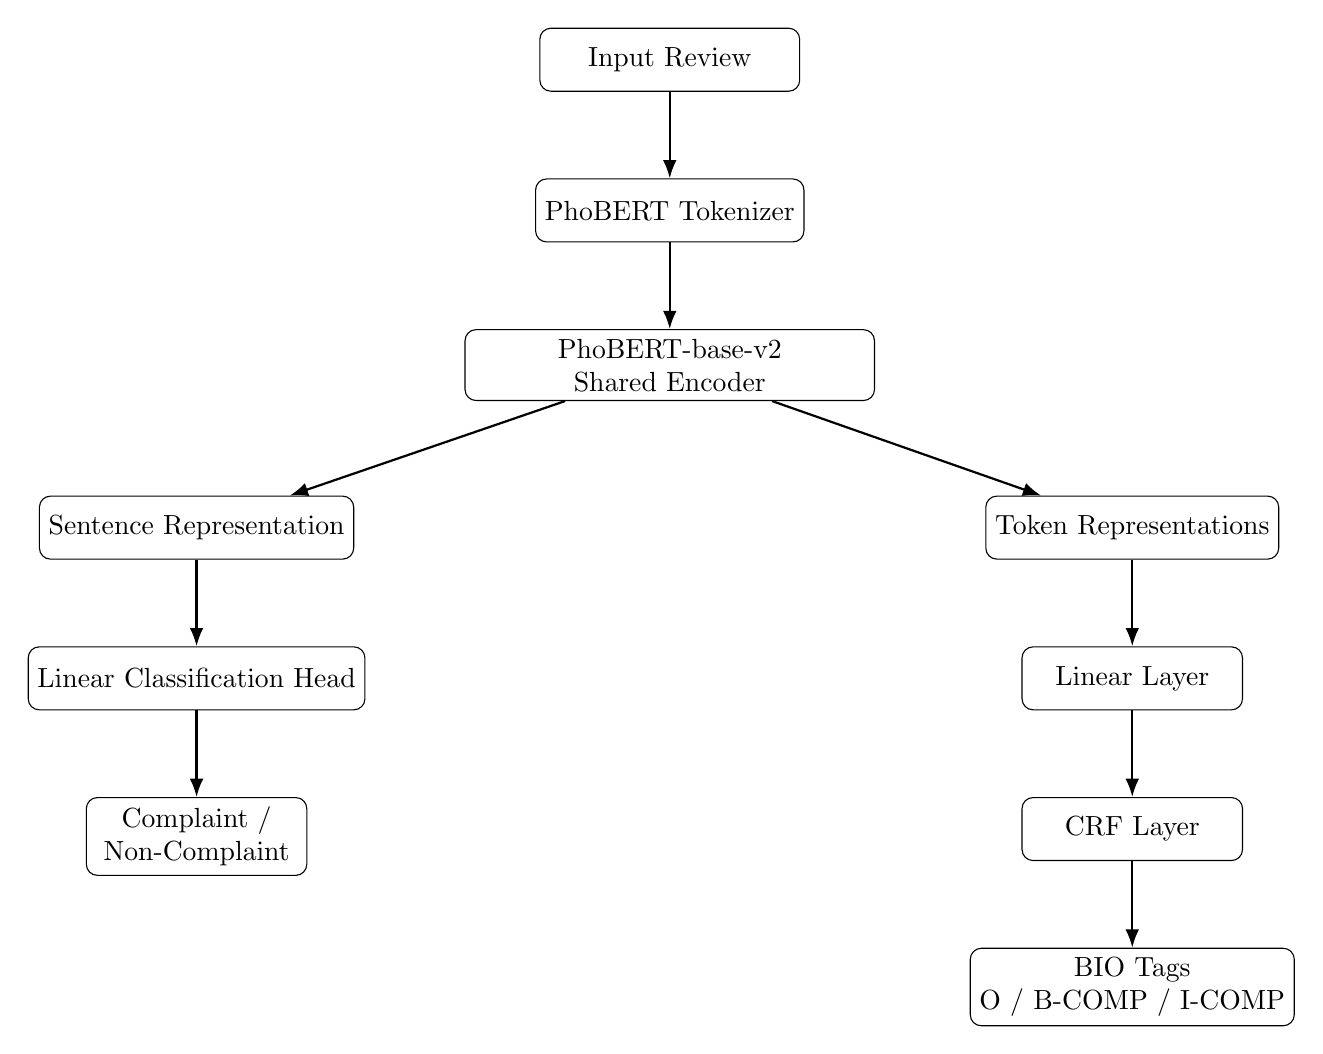
\begin{tikzpicture}[
    node distance=1.1cm,
    box/.style={rectangle, draw, rounded corners, align=center, minimum width=3.3cm, minimum height=0.8cm},
    smallbox/.style={rectangle, draw, rounded corners, align=center, minimum width=2.8cm, minimum height=0.8cm},
    arrow/.style={-Latex, thick}
]
\node[box] (input) {Input Review};
\node[box, below=of input] (tok) {PhoBERT Tokenizer};
\node[box, below=of tok, minimum width=5.2cm] (enc) {PhoBERT-base-v2\\Shared Encoder};

\node[smallbox, below left=1.2cm and 1.4cm of enc] (clsrepr) {Sentence Representation};
\node[smallbox, below right=1.2cm and 1.4cm of enc] (tokrepr) {Token Representations};

\node[smallbox, below=of clsrepr] (clshead) {Linear Classification Head};
\node[smallbox, below=of tokrepr] (linear) {Linear Layer};
\node[smallbox, below=of linear] (crf) {CRF Layer};

\node[smallbox, below=of clshead] (clsout) {Complaint /\\Non-Complaint};
\node[smallbox, below=of crf] (nerout) {BIO Tags\\O / B-COMP / I-COMP};

\draw[arrow] (input) -- (tok);
\draw[arrow] (tok) -- (enc);
\draw[arrow] (enc) -- (clsrepr);
\draw[arrow] (enc) -- (tokrepr);
\draw[arrow] (clsrepr) -- (clshead);
\draw[arrow] (clshead) -- (clsout);
\draw[arrow] (tokrepr) -- (linear);
\draw[arrow] (linear) -- (crf);
\draw[arrow] (crf) -- (nerout);
\end{tikzpicture}
\caption{Proposed Multi-task PhoBERT + CRF architecture for complaint classification and complaint span extraction.}
\label{fig:architecture}
\end{figure*}

\subsection{Training Objective}

The total training loss is a weighted combination of the classification loss and the NER loss:

\begin{equation}
L = L_{cls} + \alpha L_{ner}
\end{equation}

where \(L_{cls}\) is the cross-entropy loss for binary classification, \(L_{ner}\) is the negative log-likelihood loss from the CRF layer, and \(\alpha\) controls the contribution of the NER task. In our experiments, we evaluate two values of \(\alpha\), 1.0 and 2.0.

Since PhoBERT uses subword tokenization, label alignment is required for the NER task. For each original token, the first subword token is assigned the corresponding BIO label. The remaining subword tokens and special tokens are assigned the ignore index \(-100\), so they are excluded from loss computation.

\subsection{Implementation Details}

The proposed system is implemented using PyTorch and Hugging Face Transformers. PhoBERT-base-v2 is loaded as the shared encoder for both the classification and sequence labeling branches. For the classification task, the sentence representation is passed through a linear layer to produce logits for the complaint and non-complaint classes. For the NER task, token-level hidden states are passed through a linear projection layer before CRF decoding.

During training, each batch contains tokenized input IDs, attention masks, classification labels, and BIO labels when available. Since not all classification samples have token-level annotations, the model must handle samples with missing NER supervision. In the main experiments, we use the matched subset where both classification and NER labels are available. This setting makes the supervision consistent across the two tasks and avoids training the NER branch on unlabeled samples.

The CRF layer is used to model dependencies between adjacent BIO tags. This is useful because valid BIO sequences should follow certain structural constraints. For example, an I-COMP tag should normally appear after a B-COMP or another I-COMP tag from the same complaint span. Although the CRF layer does not completely solve the boundary detection problem, it provides a more structured decoding mechanism than independent token classification.

For evaluation and demo usage, the predicted BIO sequence is post-processed to make the output easier to interpret. Special tokens and ignored subword positions are removed from the displayed output. Consecutive B-COMP and I-COMP tags are then converted into readable complaint spans. This post-processing step is important for the Streamlit demo because users expect to see natural complaint phrases rather than subword-level predictions.

\section{Experiments}

We conduct experiments for two tasks: complaint classification and complaint span extraction. For complaint classification, we evaluate three TF-IDF-based classical machine learning baselines: Logistic Regression, LinearSVM, and Naive Bayes. The models are trained on the Shopee review dataset and evaluated on the held-out test set. The dataset is split using an 80/20 ratio, resulting in 1,564 test samples.

For complaint span extraction, we evaluate two single-task PhoBERT-based NER baselines and the proposed multi-task PhoBERT + CRF model. The first NER baseline uses PhoBERT followed by a linear token classification layer. The second baseline adds a CRF layer on top of PhoBERT to model dependencies between BIO tags. The proposed multi-task model is trained with two alpha values, 1.0 and 2.0, using the \verb|--only-ner-matched| setting because only 189 classification samples can be aligned with the NER annotations.

For classification, we report Accuracy, Macro Precision, Macro Recall, Macro-F1, and Complaint-F1. Macro-F1 is used to evaluate the overall balance between complaint and non-complaint classes, while Complaint-F1 focuses specifically on the complaint class. For NER, we report Entity Precision, Entity Recall, Entity-F1, and Token-F1. Entity-F1 evaluates exact span-level extraction, while Token-F1 measures token-level tagging performance.

All PhoBERT-based models use \texttt{vinai/phobert-base-v2} as the backbone. The models are trained with a learning rate of \(2 \times 10^{-5}\) and batch size of 8. The single-task NER baselines are trained for 5 epochs, while the multi-task models are trained for 3 epochs. Experiments are conducted on a GPU environment using Kaggle.

\begin{table}[t]
\centering
\small
\begin{tabular}{ll}
\toprule
Setting & Value \\
\midrule
Backbone & PhoBERT-base-v2 \\
Batch size & 8 \\
Learning rate & \(2 \times 10^{-5}\) \\
NER single-task epochs & 5 \\
Multi-task epochs & 3 \\
Alpha values & 1.0, 2.0 \\
Classification test size & 1,564 \\
NER test size & 100 \\
Environment & Kaggle GPU \\
\bottomrule
\end{tabular}
\caption{Experimental setup.}
\label{tab:setup}
\end{table}

\section{Result Analysis and Error Analysis}

\subsection{Classification Results}

Table~\ref{tab:classification} shows the classification results on the Shopee test set. Among the classical baselines, LinearSVM achieves the best performance with an accuracy of 0.9431, Macro-F1 of 0.9428, and Complaint-F1 of 0.9470. Logistic Regression and Naive Bayes also achieve competitive results, with Macro-F1 scores of 0.9390 and 0.9339, respectively. These results indicate that TF-IDF n-gram features are highly effective for binary complaint detection in Vietnamese e-commerce reviews.

\begin{table}[t]
\centering
\small
\begin{tabular}{lccc}
\toprule
Model & Acc. & Macro-F1 & Comp.-F1 \\
\midrule
Naive Bayes & 0.9341 & 0.9339 & 0.9381 \\
Logistic Regression & 0.9393 & 0.9390 & 0.9431 \\
LinearSVM & \textbf{0.9431} & \textbf{0.9428} & \textbf{0.9470} \\
\bottomrule
\end{tabular}
\caption{Classification results on the Shopee test set.}
\label{tab:classification}
\end{table}

\begin{figure}[t]
\centering

\includegraphics[width=\columnwidth]{figures/f1_comparison_Shopee.png}
\caption{Macro-F1 comparison of classical classification baselines.}
\label{fig:classification-f1}
\end{figure}

\subsection{NER Results}

Table~\ref{tab:ner} shows the NER results on the BIO complaint span extraction test set. The single-task PhoBERT + Linear NER and PhoBERT + CRF NER baselines achieve very low Entity-F1 scores of 0.0194 and 0.0170, respectively. Although their Token-F1 scores are higher, the entity-level performance remains poor. This suggests that the models can learn some token-level patterns but fail to extract complete complaint spans accurately.

The proposed multi-task PhoBERT + CRF model significantly improves complaint span extraction. With the \verb|--only-ner-matched| setting, the model achieves Entity-F1 scores of 0.3279 and 0.3244 for alpha values of 1.0 and 2.0, respectively. Compared with the single-task NER baselines, the improvement is substantial.

\begin{table}[t]
\centering
\small
\begin{tabular}{lcc}
\toprule
Model & Entity-F1 & Token-F1 \\
\midrule
PhoBERT + Linear NER & 0.0194 & 0.4231 \\
PhoBERT + CRF NER & 0.0170 & 0.4172 \\
MTL PhoBERT + CRF, \(\alpha=1.0\) & \textbf{0.3279} & 0.6445 \\
MTL PhoBERT + CRF, \(\alpha=2.0\) & 0.3244 & \textbf{0.6627} \\
\bottomrule
\end{tabular}
\caption{NER results on the BIO complaint span extraction test set.}
\label{tab:ner}
\end{table}

\begin{figure*}[t]
\centering

\includegraphics[width=0.38\linewidth]{figures/ner_entity_f1_comparison.png}
\hfill

\includegraphics[width=0.38\linewidth]{figures/ner_token_f1_comparison.png}
\caption{Entity-F1 and Token-F1 comparison of multi-task PhoBERT + CRF configurations.}
\label{fig:ner-f1}
\end{figure*}

\subsection{Error Analysis}

For classification error analysis, LinearSVM produces 43 false positives and 46 false negatives over 1,564 test samples. False positives often occur when a non-complaint review contains negative expressions or describes minor issues. False negatives often appear in implicit complaints or mixed-sentiment reviews, where positive and negative expressions occur in the same review. Since Shopee classification labels are derived from ratings, rating-label noise may also contribute to classification errors.

For NER error analysis, boundary detection is the main challenge. The PhoBERT + Linear NER model produces many boundary errors, suggesting that it can often identify an approximate complaint region but fails to determine the exact span boundaries. The PhoBERT + CRF model reduces boundary errors but misses most complaint entities, indicating that CRF decoding alone is insufficient when the BIO-annotated dataset is small. In the multi-task setting, Token-F1 remains higher than Entity-F1, which further confirms that the model performs better at token-level tagging than exact span extraction.

\begin{table}[t]
\centering
\small
\setlength{\tabcolsep}{4pt}
\begin{tabular}{lrrrr}
\toprule
Model & Bound. & Miss. & Spur. & Corr. \\
\midrule
Linear NER & 89 & 3 & 1 & 7 \\
CRF NER & 5 & 94 & 0 & 1 \\
\bottomrule
\end{tabular}
\caption{NER error summary for single-task NER baselines.}
\label{tab:ner-error}
\end{table}

Several factors explain the remaining errors. First, the NER dataset is small, containing only 400 training samples and 100 test samples. Second, only 189 out of 7,817 classification samples can be aligned with NER annotations, which limits the amount of token-level supervision available for multi-task learning. Third, complaint spans in Vietnamese e-commerce reviews often have ambiguous boundaries. Finally, user reviews frequently contain informal Vietnamese, spelling mistakes, abbreviations, emojis, and mixed sentiment, making both classification and span extraction more difficult.

\subsection{Qualitative Discussion}

Beyond aggregate scores, qualitative inspection shows that the span extraction task is more difficult than binary complaint classification. In many reviews, the model can identify the general region where a complaint occurs, but it may include too many or too few surrounding tokens. This explains why Token-F1 is much higher than Entity-F1. A prediction can contain several correct complaint-related tokens, but if the predicted span boundary does not exactly match the gold span, the entity-level metric still counts it as incorrect.

Boundary errors are especially common in reviews with mixed sentiment. For instance, a review may contain a positive phrase such as ``san pham dep'' followed by a negative phrase such as ``giao hang cham''. In this case, the model must separate the positive part from the complaint part. If it includes the positive phrase in the complaint span, the extracted entity becomes too long. If it only predicts ``cham'' instead of ``giao hang cham'', the extracted entity becomes too short. Both cases reduce Entity-F1 even though the model captures part of the complaint meaning.

Missed entities are another important error type. These errors often occur when complaints are expressed indirectly or without strong negative keywords. For example, a review such as ``lan sau chac minh khong mua nua'' expresses dissatisfaction, but it does not explicitly mention a product defect or service problem. Such implicit complaints are difficult for both classification and span extraction models. They require pragmatic understanding beyond simple keyword matching.

These observations suggest that future improvements should focus not only on model architecture but also on annotation quality and data coverage. More BIO-annotated samples would help the model learn diverse span boundaries. In addition, consistent annotation guidelines are important because ambiguous span boundaries can make training and evaluation unstable. This is particularly important for Vietnamese e-commerce reviews, where users often write short, informal, and noisy comments.

\subsection{Demo System and Reproducibility}

To demonstrate the practical usage of the proposed approach, we build a Streamlit-based demo system. The demo allows users to input a Vietnamese e-commerce review and receive two types of outputs: the predicted complaint classification label and the extracted complaint spans. The interface also highlights the extracted spans in the original review, making the output easier to understand for non-technical users.

The demo checkpoint is selected based on the NER performance of the multi-task PhoBERT + CRF model. Therefore, the system is mainly optimized to demonstrate complaint span extraction rather than perfect binary classification. In some short positive reviews, the classification branch may produce false-positive predictions. To make this limitation explicit, the demo shows a warning when the model predicts a complaint but no complaint span is extracted. This design choice prevents the system from over-interpreting uncertain predictions.

The demo also includes token-level BIO details for debugging and analysis. This view is useful for inspecting whether the model correctly identifies the beginning and continuation of complaint spans. For example, given the review ``shop giao hang qua cham, san pham bi mop meo'', the system can identify ``giao hang qua cham'' and ``bi mop meo'' as complaint spans. Such visualization helps connect the quantitative NER results with qualitative model behavior.

In addition to the demo interface, the project is organized with separate scripts for preprocessing, training, evaluation, metric collection, and error analysis. This structure improves reproducibility and makes it easier to rerun individual components of the pipeline. The final system therefore includes not only trained models, but also a complete experimental workflow from raw review data to evaluation reports and interactive demonstration.

\section{Conclusion and Future Work}

In this study, we proposed a PhoBERT-based multi-task learning approach for Vietnamese complaint detection and complaint span extraction in e-commerce reviews. The proposed model jointly performs sentence-level complaint classification and token-level complaint span extraction. PhoBERT-base-v2 is used as the shared encoder, while two task-specific heads are designed for binary classification and BIO sequence labeling with CRF.

Experimental results show that classical TF-IDF-based models are highly effective for binary complaint classification. In particular, LinearSVM achieves the best classification performance with an accuracy of 0.9431, Macro-F1 of 0.9428, and Complaint-F1 of 0.9470 on the Shopee test set. However, such models only provide sentence-level predictions and cannot identify the specific complaint phrases inside reviews.

For complaint span extraction, single-task PhoBERT-based NER models perform poorly, achieving Entity-F1 scores of only 0.0194 and 0.0170. In contrast, the proposed multi-task PhoBERT + CRF model substantially improves NER performance. The alpha=1.0 configuration achieves the highest Entity-F1 score of 0.3279, while the alpha=2.0 configuration achieves the highest Token-F1 score of 0.6627. These results suggest that jointly learning complaint classification and complaint span extraction can improve token-level and span-level complaint understanding when BIO-annotated data is limited.

In future work, we plan to expand the BIO-annotated dataset using semi-automatic labeling and active learning. We also aim to improve the alignment between classification and NER data using fuzzy matching or embedding-based matching. More comprehensive ablation studies with different alpha values, training strategies, and model variants should be conducted. Finally, deeper error analysis across product domains can help improve the robustness of complaint detection and complaint span extraction systems in real-world e-commerce applications.

\section*{Limitations}

The proposed approach still has several limitations. First, the BIO-annotated NER dataset is small, containing only 400 training samples and 100 test samples. Second, only 189 out of 7,817 classification samples can be aligned with NER annotations, which limits the amount of token-level supervision available for multi-task learning. Third, complaint span boundaries are ambiguous in Vietnamese e-commerce reviews, especially when reviews contain informal language, spelling errors, abbreviations, emojis, or mixed sentiment. Finally, the classification labels in the Shopee dataset are derived from product ratings, which may introduce label noise.

% Custom bibliography entries only
\bibliography{custom}

\end{document}
```
